\documentclass[a4paper]{article}

\usepackage{amsmath, graphicx, float, blindtext} % for dummy text
\graphicspath{ {./images/} }
\title{Null Hypothesis Significance Testing}
\author{Shubham Gupta}

\begin{document}
\maketitle

\section{Introduction}
\begin{itemize}
    \item Goal of NHST: Determine if a particular value for a parameter can be rejected.
    \item Probability of getting an outcome from the null hypothesis that is as extreme as the observed outcome is called the `p` value.
    \item If \text{p value} is very small, we reject the outcome.
    \item Single outcome can have multiple p values depending on the sampling intention.
    \item Stopping at a fixed number of flips or after a fixed duration \textbf{does not} bias the data. Stopping after getting a fixed number of flips \textbf{does} bias the data.
\end{itemize}
\section{p value}
\begin{itemize}
    \item We will compute p value with the bayes formula:
        \[
            \text{pvalue} = likelihood * prior
        .\] 
    \item \textbf{Likelihood function}: Probability for a single measurement AND the intended sampling process that defines space of all possible outcomes.
    \item \textbf{Null hypothesis}: Likelihood function with a specific value of $\theta$.
    \item All possible values are defined by $I$.
    \item Each sample from the null hypothesis is given by  $D_{\theta, I}$.
    \item For coin null hypothesis,  $D_{\theta, I}$ will be $ \frac{z}{N}$.
    \item \textbf{Sampling distribution}: Probability distribution over all possibilities i.e $p(D_{\theta, I}|\theta, I)$.
    \item \textbf{Expected value}: Typical value of $p(D_{\theta, I}|\theta, I)$ i.e $E[D_{theta, I}]$
        \[
            pvalue = p(D_{\theta, I} \text{ } fancysymbol \text{ } D_{actual}|\theta, I)
        .\]  
        \begin{figure}[H]
            \centering
            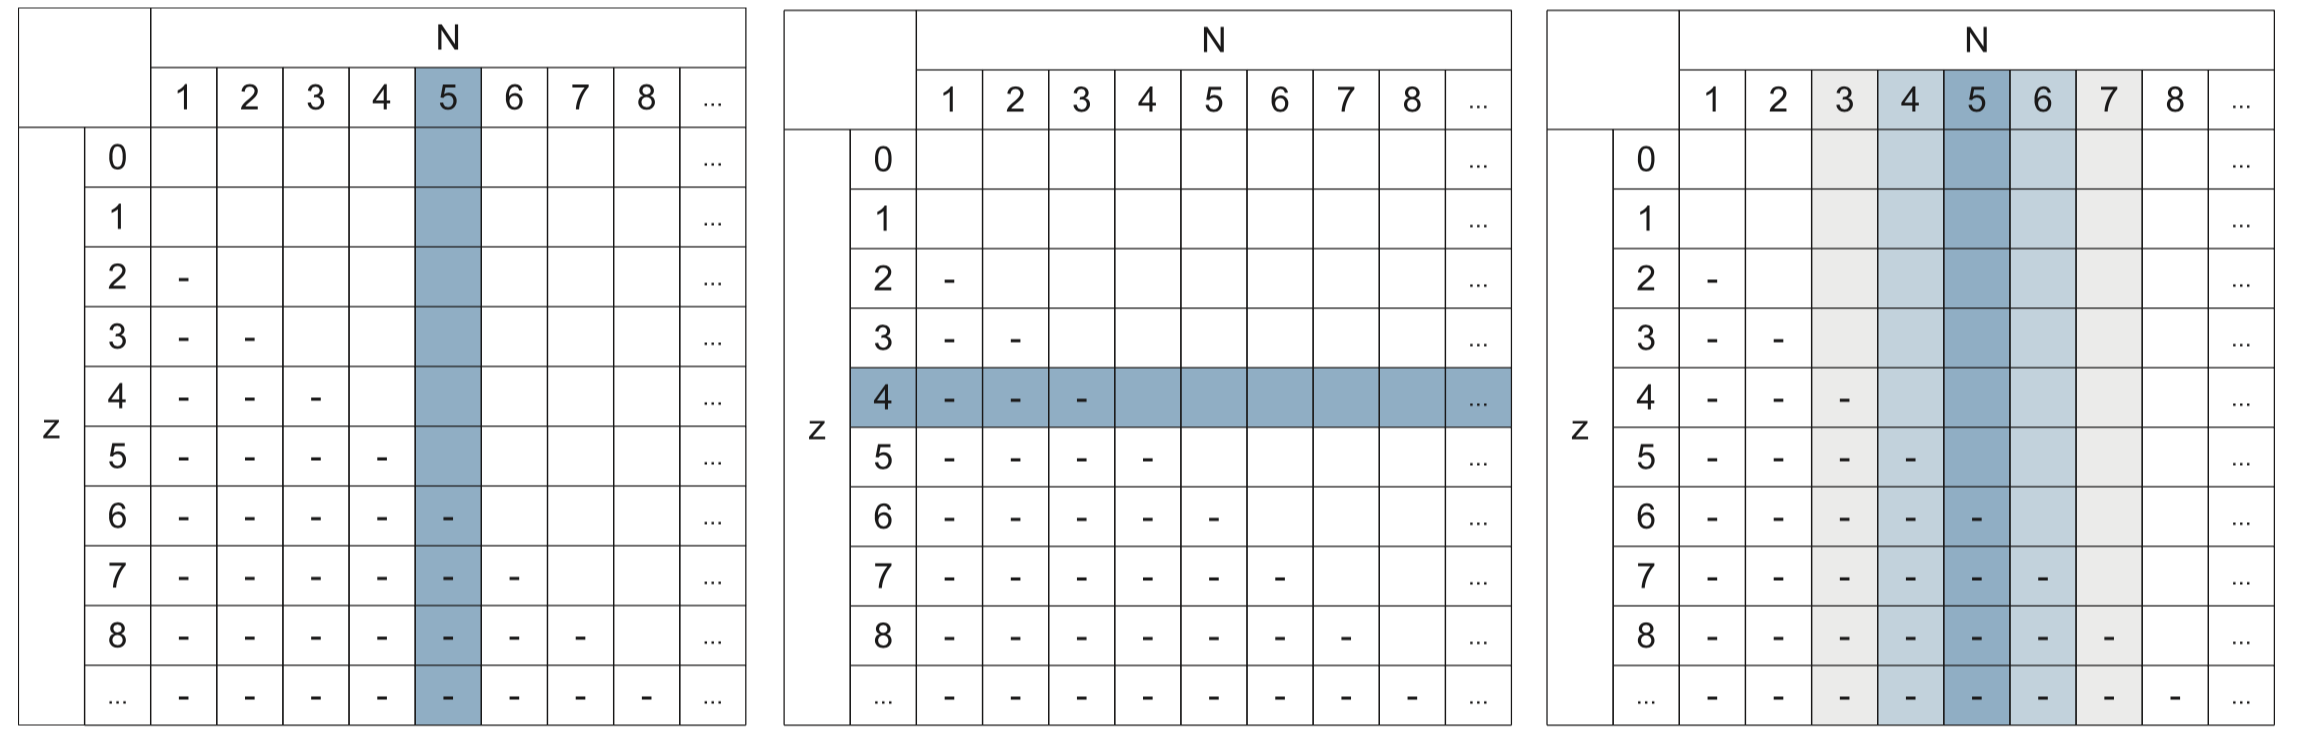
\includegraphics[width=0.8\textwidth]{possible_outcomes}
            \caption{Space sample for coin flips. Left: Fixed N. Middle: Fixed z Right: Fixed time duration}
            \label{fig:possible_outcomes}
        \end{figure}
\end{itemize}
\subsection{Intention to fix $N$ }
\begin{itemize}
    \item When $N$ is fixed, it will represent the left table.
    \item \textbf{Aim}: What is the probability of $z$ when $N$ is fixed?
    \item \textbf{Answer}: Binomial distribution 
        \[
            p(z|N, \theta) = \binom{N}{z} \theta^{z} (1-\theta)^{N-z}
        .\]
        \begin{figure}[H]
            \centering
            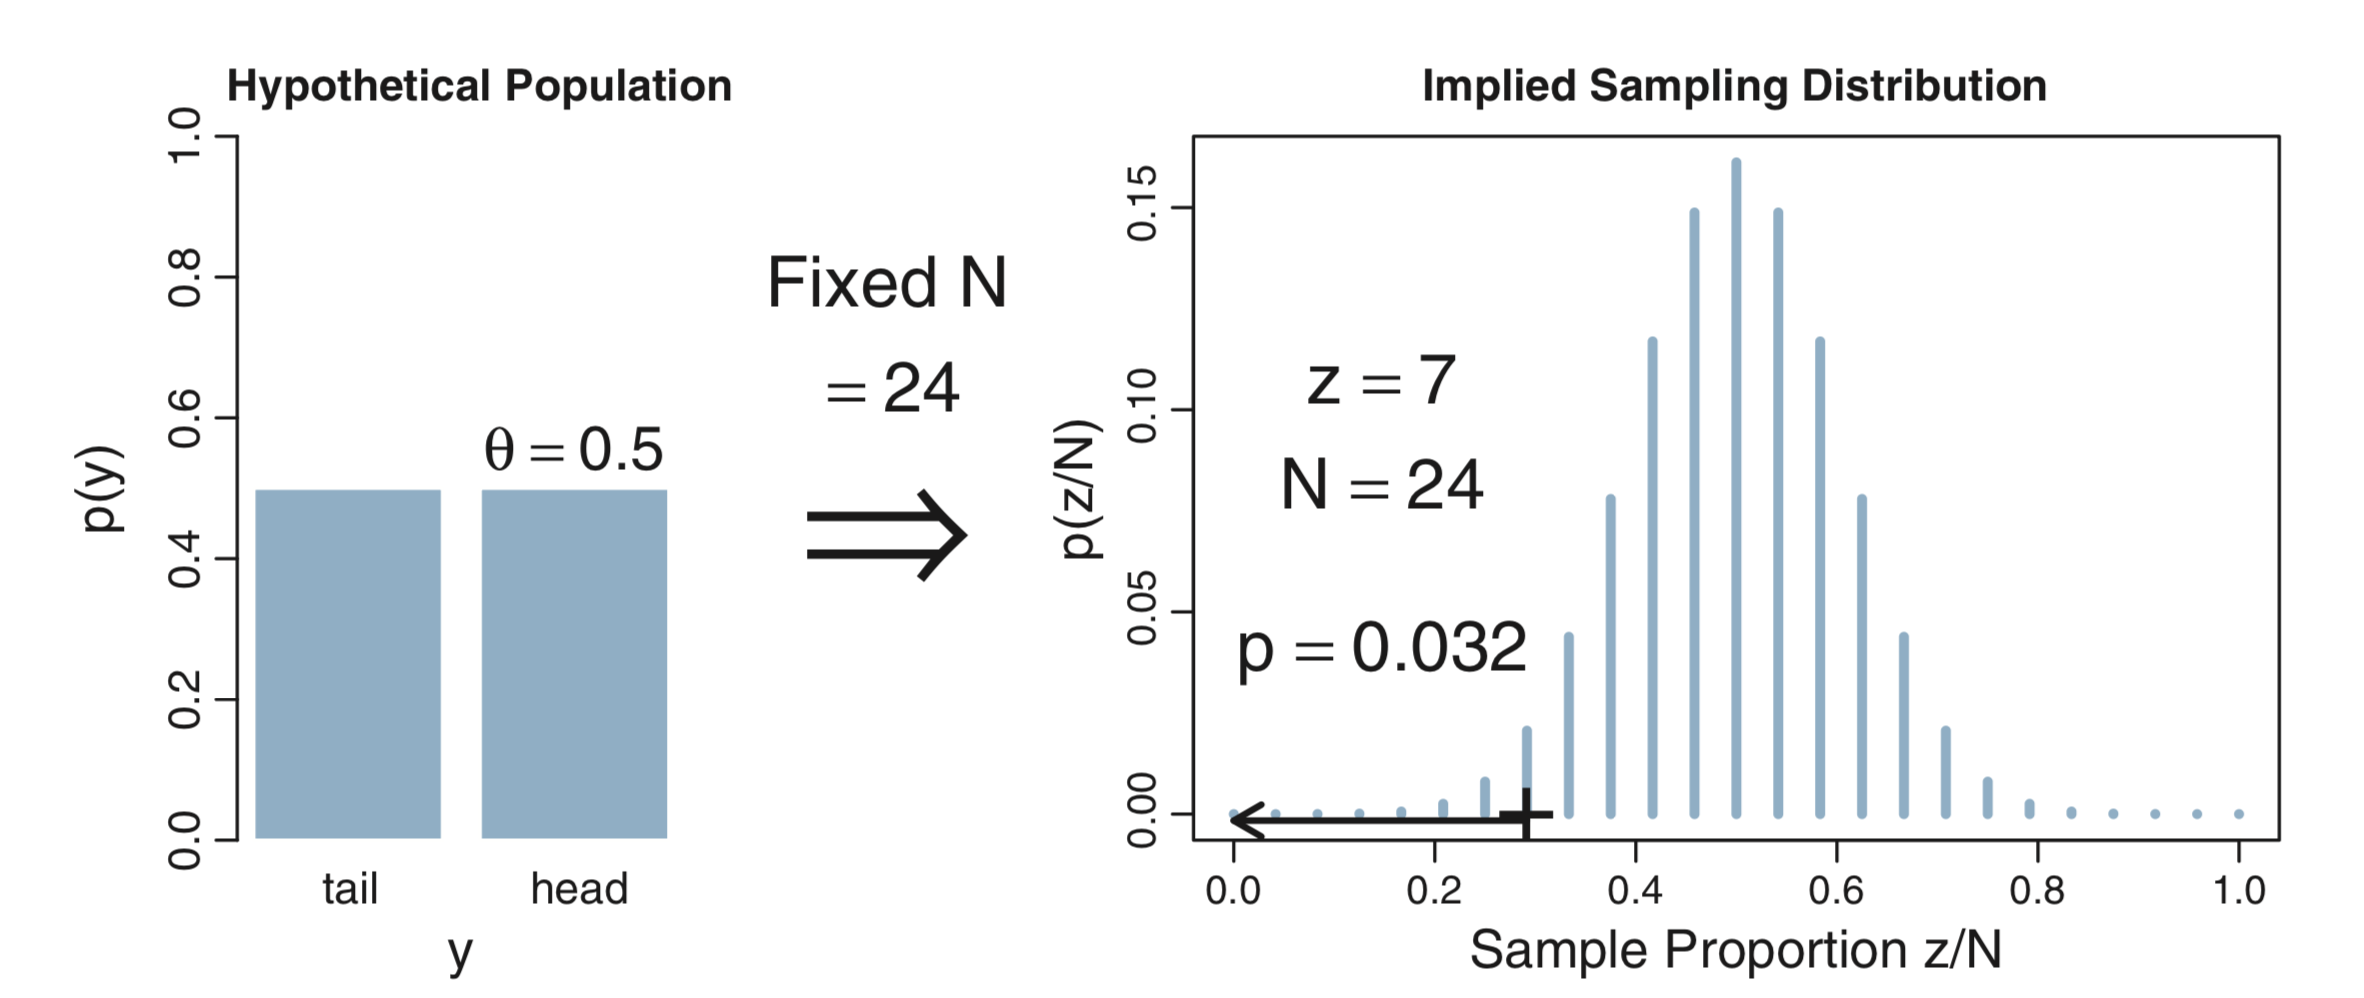
\includegraphics[width=0.8\textwidth]{binomial_sampling_distribution}
            \caption{Binomial distribution i.e Sampling distribution}
            \label{fig:binomial_sampling_distribution}
        \end{figure} 
    \item We will get the above sampling distributions where there are infinitiely many samples performed.
    \item Sampling distribution is probability distribution over samples of data, \textbf{not over values of theta.}  
    \item p-value is conventially set to 5\%.
    \item We will compute p-value using the following:
        \[
            p(\text{right tail}) = p((z/N)_{\theta, I} \geq (z/N)_{actual}|\theta, I)
        .\] 
        \[
            p(\text{left tail}) = p((z/N)_{\theta, I} \leq (z/N)_{actual}|\theta, I)
        .\] 
    \item For the given example, we get the one-tailed p-value as 3.2\%. Since it is larger than 2.5\%(p-value for one tailed distribution. For two tailed it will be the conventional 5\%), we \textbf{do not} reject the null hypothesis. 
\end{itemize}
\subsection{Intention to fix $z$ }
\begin{itemize}
    \item Calculate probability of the process taking $N$ flips to get $z$ heads. 
    \item We know $ N$th flip got the $z$ head.
    \item $N-1$ flips had $z-1$ heads.
    \item Using binomial distribution, probability of $z-1$ heads in $N-1$ flips is:
        \[
            \binom{N-1}{z-1}\theta^{z-1}(1-\theta)^{N-z}
        .\] 
    \item Probability of getting heads in last flip is $\theta$.
    \item Therefore, we get:
        \[
            \binom{N-1}{z-1}\theta^{z-1}(1-\theta)^{N-z}* \theta
        .\]         
        \[
            =     \frac{z}{N} \binom{N}{z}\theta^{z}(1-\theta)^{N-z}
        .\] 
    \item This is called the \textbf{negative binomial distribution}  
        \begin{figure}[H]
            \centering
            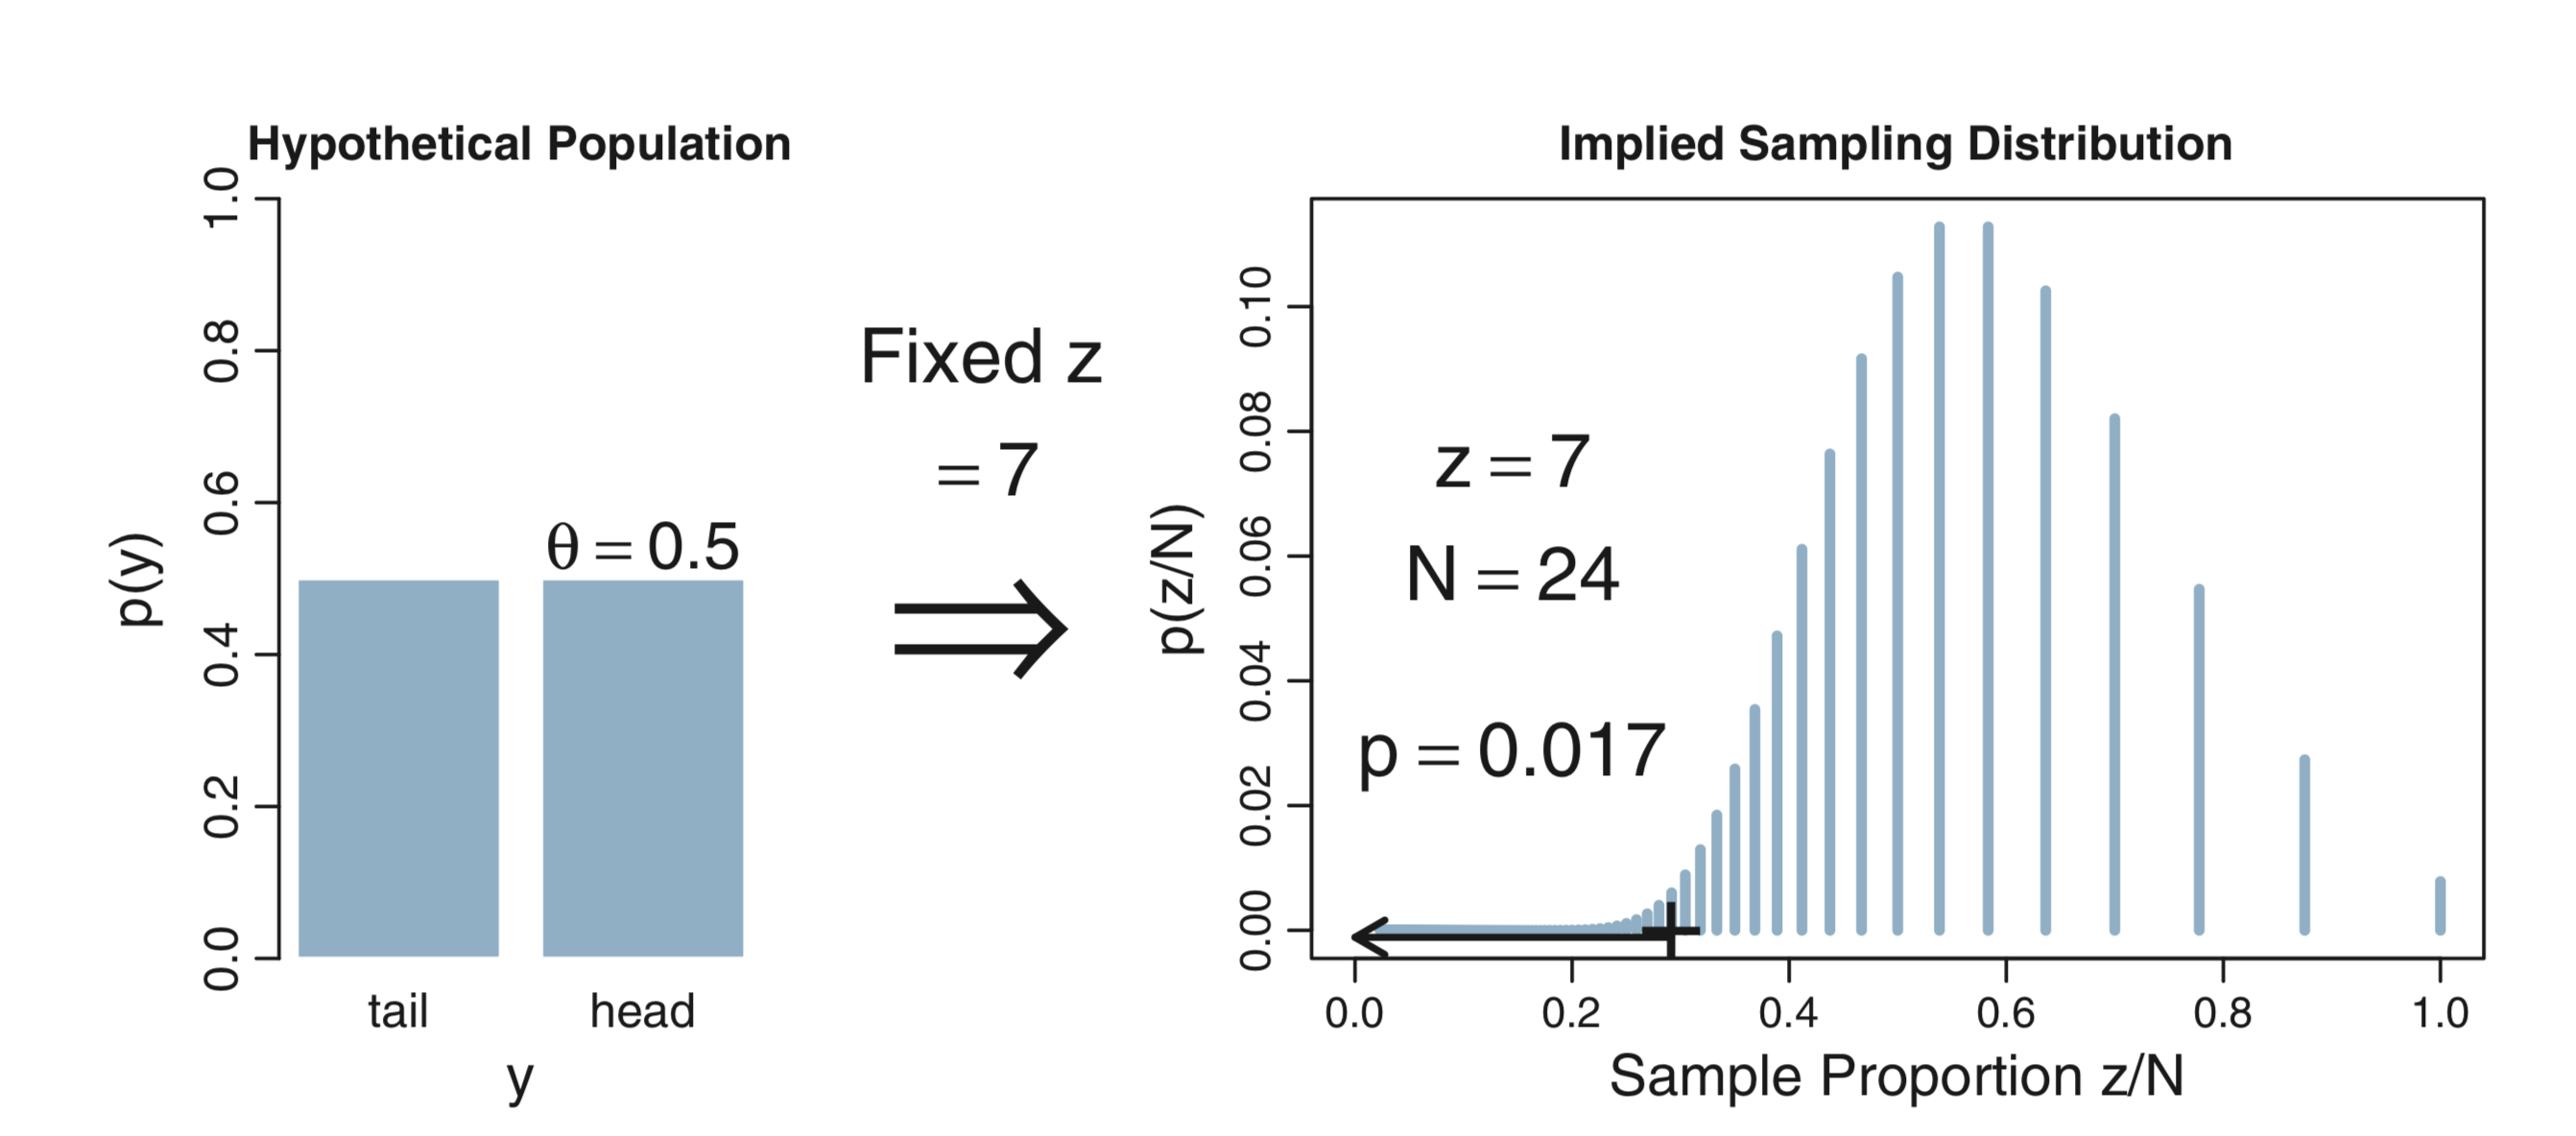
\includegraphics[width=0.8\textwidth]{nbd_distribution}
            \caption{Sampling distribution for fixed $z$}
            \label{fig:nbd_distribution}
        \end{figure}
    \item When $N=7$ and $z=7$, we get the spike at 1.0
    \item When $N=8$ and $z=7$, we get the spike at 0.875
    \item Spikes at left tail become dense and short as the value of $N$ increases.
    \item Since $pvalue=0.017$ is less than threshold of $2.5\%$, we reject the null hypothesis.
    \item \textbf{pvalue varies for different sampling scenarios.}
\end{itemize}
\subsection{Intention to fix duration}
\begin{itemize}
    \item Neither $z$ or $N$ will be fixed.
    \item We need to specify how various combos of $N $ and $ z$. 
    \item $N$ can be small or large depending on the speed of sampling. Hence, we will use a \textbf{Poisson distribution}. 
    \item Poisson distribution has a parameter $\lambda$, which is the mean value(and also the variance).
    \item For every value of $N$, the $z$ values are binomial distributions. Hence, a Poisson distribution is a \textbf{mixture of binomial distributions}  
\end{itemize}
\end{document}
